\documentclass[]{article}
\usepackage[xcolor]{changebar} 
\usepackage{hyperref}
\usepackage{cleveref}
\usepackage{listings}
\newcommand{\deleted}[1]{%
	\cbcolor{red}
	\begin{changebar}
		#1
	\end{changebar}%
}%

\newcommand{\added}[1]{%
	\cbcolor{green}
	\begin{changebar}
		#1
	\end{changebar}%
}%
\usepackage{tikz}
\usetikzlibrary{automata,positioning,arrows}

%opening
\title{Automatic extraction of symbolic network signatures from malware code}
\author{Arjun Gurumurthy, Kausik Subramanian}

\begin{document}

\maketitle

\begin{abstract}
We propose the automatic extraction of symbolic network signatures from malware code to aid and automate network-based malware detection systems.
\end{abstract}

\section{Motivation}
Malware, short for malicious software, 
is one of the primary threats to modern-day networks, especially
with the mass proliferation of the Internet. These are used to 
disrupt computer operations, extract sensitive information, and 
gain access to private systems.  Infected hosts can participate 
in distributed denial-of-service attacks (DDoS), these class of 
attacks are very hard to detect and mitigate, leading to immense
loss of revenues. A new shift is towards creating malware for 
profit called botnets, in which a customer can buy a network of
infected hosts for a price. In such a setting, the malware is
specifically designed to evade detection, thus motivating the need
for better detection tools for malware. 

The most prevalent form of malware detection is endhost-based detection
(commonly known as anti-virus software). Detected malware's code is hashed
and the code signatures are uploaded to a central repository. By maintaining
an up-to-date repository of malware signatures, the endhost software can
detect malware by comparing program signatures with the repository. However, 
endhost-based malware detection can fail due to various reasons~\cite{networksig}:
\begin{itemize}
	\item \textbf{Anti-virus software is not operational or up to date.} 
	Due to this, the endhost machine can be infected by malware without any
	noticeable effects, thus the user will be oblivious of the infection.
	\item \textbf{Packer programs.} To render programs stealthy, malware authors
	employ packer programs~\cite{packer}. Packers change the program content so that
	its signature differs but its functionality has not changed, thus avoiding
	detection by endhost signature-based software.
\end{itemize}

Instead, a intrusion-detection mechanism integrated 
directly into the service provider’s network offers a
much-needed additional layer of protection. While the malware
code is different, the protocol of the malware used to talk to its
control server (which issues orders to the malware) will not vary. 
Thus, by generating accurate \emph{network signature} of the malware (which
can informally defined as the set of messages sent and received by the malware to
initiate an action), we can use the intrusion detection system in the
network (for e.g., Bro~\cite{bro}) to search for these particular signatures,
and can be used to infer the presence of the malware in the network. However,
manually inspecting malware code is an intractable approach (signatures may 
need to be extracted in real-time). Thus, we propose \emph{automatic extraction 
of accurate network signatures from malware code using different static
analysis techniques.} 

\section{Challenges}
We abstract the problem to the following: given a program point,
can we automatically provide an ordered set of symbolic packets 
that must be received (and sent) by the client such that the program 
reaches the program point. The symbolic packets can be used as
network signatures and used to detect malware (a set of packets
satisfying the symbolic packets in order will infer that there 
is a malware with high confidence). By constructing symbolic packet
signatures, we can generalise the intrusion policy and reduce 
true negatives (thus not affecting legitimate traffic).

Malware code can be thought of as a program reacting based on input received
packets received (possibly multi-threaded), which
could require changes to existing reachability analyses tools 
like Codesurfer~\cite{codesurfer}. To extract symbolic network
signatures, we need to define the abstract semantics of the program
suited for network signatures, and define the \emph{combine} and 
\emph{extend} operators used for interprocedural analysis.

\section{Project Proposal}
\textbf{Tasks}:
\begin{itemize}
	\item Identify and characterize features of common malware code - 1-2 weeks
	\added{Refer to sections A and B}
	\item \deleted{Develop the abstract semantics and operators for extracting  
	symbolic network signatures from malware code - 2-3 weeks} \\
	\added{Automatically generate a symbolic automaton of the given program
		based on packet and variable state - 2-3 weeks}
	\item Modifying/Extending existing tools like Codesurfer for symbolic 
	network signature extraction - 2-3 weeks
\end{itemize}

\noindent\textbf{Open source tools}: Static analysis tools, malware repositories

\noindent\textbf{Evaluation}: 
The primary metrics of evaluation are time taken for analysis, accuracy and 
generality of the symbolic signatures. Performance analysis can be performed 
with different malware programs with varying lines of code to understand
the time complexity of the analysis. The quality of the symbolic network
signatures is a tougher metric to measure. Ideally, the symbolic network 
signature must only include packets which will make the program reach the
specified point. If the signature is more general, legitimate packets may 
be considered as malicious and blocked. On the other hand, the signature
may miss actual malware traffic because the signature does not encompass
all inputs leading to the point. We would try to address these trade-offs in
our evaluation.

\appendix
\section{Malware program model}
The malware program listens to incoming packets, and the
network signature is the set of incoming packets which triggers
an attack by the program. We propose a reasonable abstraction
of the code of malware programs. 

We model a malware program as a infinite reactive system 
of the form:
\begin{lstlisting}	
while(True) {
	packet = socket.receive();
	...
}
\end{lstlisting}
Each iteration of the loop, the program receives a
packet, and based on current state and packet received,
it performs certain actions. Using static analysis
techniques, we can identify two set of variables, \emph{state}
and \emph{packet} variables. State variables represent the 
program state in terms of the protocol, which packet variables
are used to represent the current packet being processed by
the program.
\begin{lstlisting}	
while(True) {
	packet = socket.receive();
	...
	if (a == 1 and packet[8] = "b") {
		a = a + 1;
	}
	...
}
\end{lstlisting}	
In the above code snippet, $a$ is a state variable
and $packet$ is a packet variable. This also
illustrates the packet processing 
function of the program, which based on the current
input packet and state variables, either transitions
to a new program state or performs an action (attack or
send packets). 
\begin{lstlisting}	
a = 0;
while(True) {
packet = socket.receive();
	if (a == 0 and packet[0] = "a") {
		a = a + 1;
	}
	if (a == 1 and packet[0] = "b") {
		a = a + 1;
	}
	if (a == 2 and packet[0] = "c") {
		attack()  [the attack point is provided as 
				input to analysis]
	}	
}
\end{lstlisting}	
The above code snippet represents the complete model
of the malware program, where based on input packets and
current state, the program transitions to a new state. 
The symbolic automaton for this program is 
shown in \Cref{fig:progautomaton}. Network signatures
for the malware are all paths from start state ($a=0$)
to state of attack. In this case, the sequence of packets
in order to initiate an attack is $a* \rightarrow b* \rightarrow c*$.
\begin{figure}[h]
	\centering
	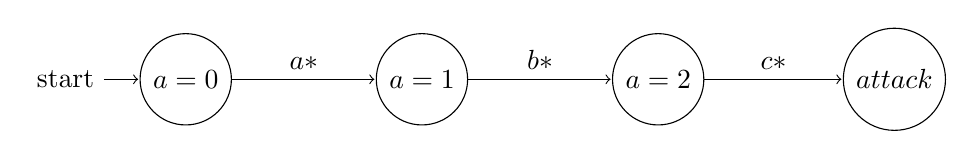
\begin{tikzpicture}[shorten >=0.5pt,node distance=3cm,on grid,auto] 
	\node[state, initial] (v0)   {$a = 0$}; 
	\node[state] (v1) [right=of v0] {$a = 1$}; 
	\node[state] (v2) [right=of v1] {$a = 2$};
	\node[state] (v3) [right=of v2] {$attack$}; 	
	\path[->] 
	(v0) edge node {$a*$} (v1)
	(v1) edge node {$b*$} (v2)
	(v2) edge node {$c*$} (v3);
	\end{tikzpicture}
	\caption{Symbolic automaton for malware program.}
	\label{fig:progautomaton}
\end{figure}

\section{Related Work}
An important assumption that we make is that of the simplification of the botnet client code to a set of \textbf {if (state, packet)} statements. Looking at existing research, significant work has gone into automatic protocol reverse-engineering of botnet C\&C protocols using dynamic binary analysis based on network traces. This generally follows a two step process: Extract the protocol grammar, that captures the structure of messages comprising the protocol. Knowing the protocol message format would enable the construction of the protocol state machine, which represents the sequence of messages as a specification of protocol states and transition between states (based on messages received). 
For example, Polyglot~\cite{polyglot} is a system that uses dynamic binary analysis to automatically extract the protocol message format, and Dispatcher~\cite{dispatcher} is a tool that makes use of techniques specified in Polyglot to extract the message format and field semantics for messages sent and received by the application.

Taint propagation is used by the tool to map how the packets received manipulate the state. When the program calls the \textit{read()} function, Dispatcher uses the function's prototype to determine if any argument is tainted based on the memory locations it accesses. Via this approach, a spam botnet called MegaD is analyzed by Dispatcher.

Thus, having knowledge of the network packets received would enable us to make inferences on how they could transition to an 'attack point'. Our work focuses on static analysis of the malware code, without having to execute it and/or capture network traces.

In addition, work has been done on inferring state machines automatically for stateful network protocols - Prospex~\cite{prospex}. Prospex essentially performs clustering of similar network messages and tracks protocol state changes. By merging similar states, a minimal state machine is produced, and the paper produces a labeled state tree for the Agobot malware. This could be used as our initial malware program model for which we determine the sequence of packets to initiate an attack.


\bibliographystyle{abbrv}
\bibliography{references}

\end{document}
